\begin{frame}{\LaTeX, que no látex}
    
    \begin{block}{¿Qué es?}
        Sistema de \textbf{composición de textos} orientado a la creación de documentos escritos de \textbf{alta calidad tipográfica}, cuyo uso mayoritario es la creación de \textbf{documentos científicos} (artículos y libros).

        \LaTeX{} es un software libre bajo la \textit{Latex Project Public License - LPPL}
    \end{block}
    
\end{frame}

\begin{frame}{\LaTeX, que no látex}
    \begin{columns}
        \column{0.5\textwidth}

        \begin{block}{Bits de historia\ldots{}}
            \begin{itemize}
                \item Creado por Leslie Lamport (\textbf{Turing 2013}) en 1984 \ldots{}
                \item es el sucesor de TeX creado por Donald Knuth (\textbf{Turing 1974}) en 1978 (*)
                \item \LaTeX{}: Lamport TeX
                \item TeX: $\tau\epsilon\chi$ ('skill', 'art', 'technique')
                \item \textit{The \LaTeX{} Project} desarrollando \LaTeX{}3 
            \end{itemize}
        \end{block}
        \pause
        \column{0.5\textwidth}
            \hspace{0.5cm}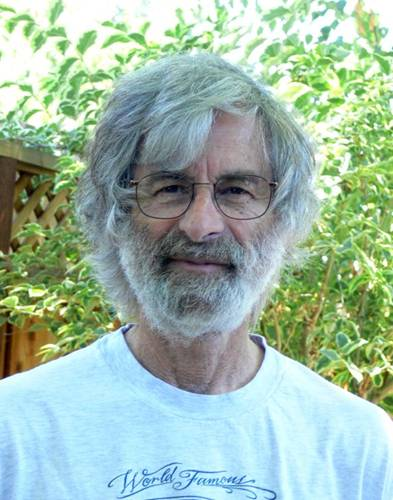
\includegraphics[width=0.8\textwidth]{images/leslie.jpg}
    \end{columns}

\end{frame}

\begin{frame}{\LaTeX, que no látex}
    \begin{columns}
        \column{0.5\textwidth}

        \begin{block}{Bits de historia\ldots{}}
            \begin{itemize}
                \item Creado por Leslie Lamport (Turing 2013) en 1984 \ldots{}
                \item es el sucesor de TeX creado por Donald Knuth (Turing 1974) en 1978 (*)
                \item \LaTeX{}: Lamport TeX
                \item TeX: $\tau\epsilon\chi$ ('skill', 'art', 'technique')
                \item \textit{The \LaTeX{} Project} desarrollando \LaTeX{}3 
            \end{itemize}
        \end{block}

        \column{0.5\textwidth}
            \hspace{0.5cm}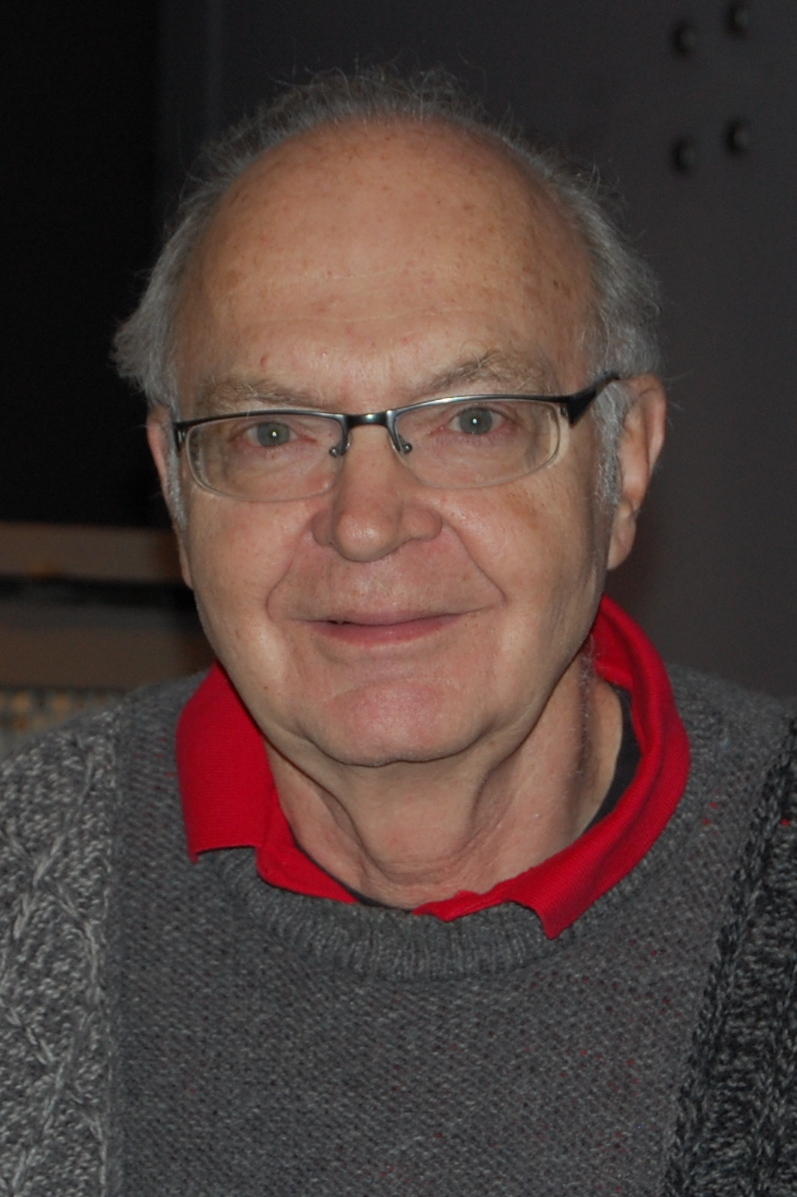
\includegraphics[width=0.8\textwidth]{images/knuth.jpg}
    \end{columns}
\end{frame}